\def\QRCODE{TB_IPR_TUT.IMG.shape_diagrams_matlabqrcode.png}
\def\QRPAGE{http://www.iptutorials.science/tree/master/TB_IPR/TUT.IMG.shape_diagrams/matlab}
\mcorrectionsection{Matlab correction}


\subsection{Geometrical functionals}
The Crofton perimeter and Feret diamaters have been already computed in the tutorial\iflabelexists{tutorial:integral_geometry:enonce}{ \ref{tutorial:integral_geometry:enonce}}{ about integral geometry.} For computing the perimeter, we use the \minline{regionprops} function.

\begin{matlab}
% classical perimeter
if (~islogical(I))
    perim = regionprops(I>100, 'Perimeter');
else
    perim = regionprops(I, 'Perimeter');
end
p = perim.Perimeter;
\end{matlab}

The Crofton is evaluated with the use of 4 directions.
\begin{matlab}
I=double(I);
inter = zeros(4,1);
for i=1:4
    I2=imrotate(I, 45*(i-1));
    h=[1 -1];
    I3=conv2(I2, h, 'same')>0;
    inter(i) = sum(I3(:));
end

% formula of the Crofton perimeter
crofton = pi/4*(inter(1)+inter(3) + (inter(2)+inter(4))/sqrt(2));
\end{matlab}

The Feret diameter corresponds to the projected length in a given direction. The following code uses a angular step of 30 degrees. It computes the maximum and the minimum at the same time.
\begin{matlab}
function [d,D] = feret(I)

d=max(size(I));
D=0;
for a=0:30:179
    I2 = imrotate(I, a);
    F=max(I2);
    mesure=sum(F>0);
    
    if (mesure<d)
        d=mesure;
    end
    if (mesure>D)
        D=mesure;
    end
end
\end{matlab}

The radius of the inscribed circle can be computed as:
\begin{matlab}
function r=InscribedCircleRadius(I)
dm = bwdist(~(I>0));
r=max(dm(:));
\end{matlab}


\subsection{Morphometrical functionals}
The different morphometrical functionals can be easily computed as ratios of geometrical functionals.

\subsection{Shape diagrams}
The following process gives 3 shape diagrams for the whole Kimia image database:
\begin{matlab}
name={'apple-' 'bone-' 'camel-'};
couleur={'r+' 'g*' 'bo'};
format='.bmp';
indices=1:20;

% number of diagrams:
N_diag=3;
x=zeros(N_diag, length(name)*length(indices));
y=zeros(N_diag, length(name)*length(indices));

xlabs={'\omega/d' '\omega/d' '2*r/d'};
ylabs={'2*r/d' '4A/(pi*d^2)' 'P/(pi*d)'};

% computation of the functionals for all the images
for n=1:length(name)
    for i=indices
        
        I = imread([name{n} num2str(i) format]);
        [omega d] = feret(I);
        [crofton, P] = perimetres(I);
        r = rayonInscrit(I);
        stats = regionprops(I>0, 'Area');
        ii = (n-1)*length(indices)+i;
        x(1,ii)=omega/d;
        x(2,ii)=omega/d;
        x(3,ii)=2*r/d;
        
        y(1,ii)=2*r/d;
        y(2,ii)=4*stats.Area/(pi*d^2);
        y(3,ii)=P/(pi*d); % values > 1, non-convex objects
        
        % progress bar
        waitbar(((n-1)*length(indices)+i)/(length(name)*length(indices)));
    end
end
\end{matlab}


The visualization is done via the following code and displayed in Fig.\ref{fig:shape_diagrams:matlab:shapeDiagrams}.

\begin{matlab}
% visualization of the 3 diagrams with a specific color for each category
for j=1:N_diag
    figure(); hold on
    for i=1:length(name)
        i1=length(indices)*(i-1)+1;
        i2=length(indices)*i;
        plot(x(j,i1:i2), y(j,i1:i2),[ couleur{i} ]); 
        
    end
    legend(name);
    xlabel(xlabs{j});
    ylabel(ylabs{j});
end
\end{matlab}    

\begin{figure}[htbp]
 \centering
 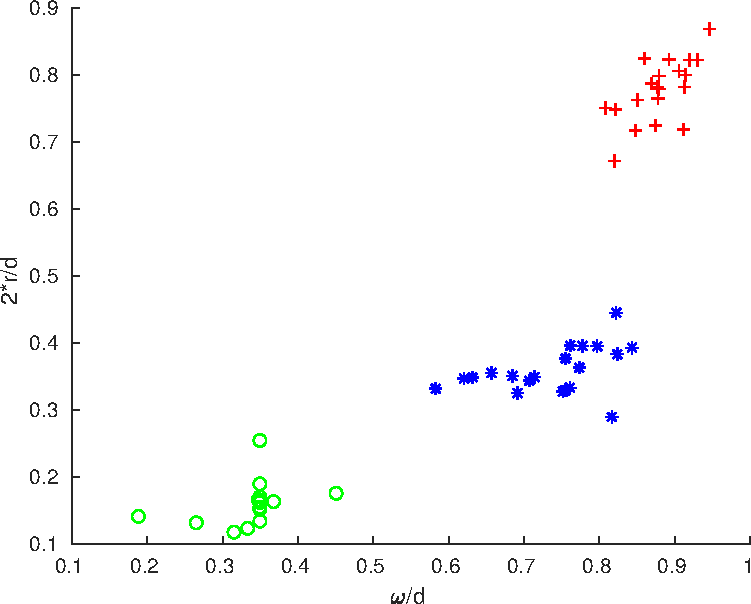
\includegraphics[height=.3\textheight]{diag1.pdf}
 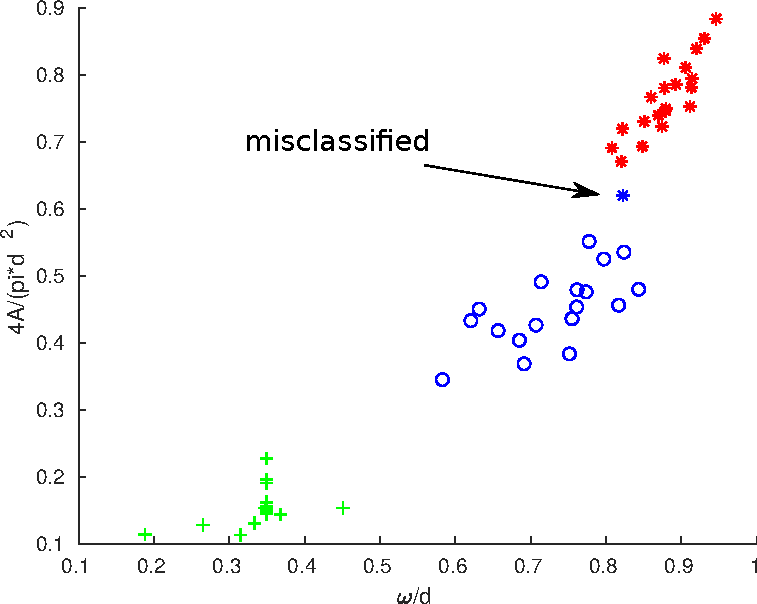
\includegraphics[height=.3\textheight]{diag2.pdf}
 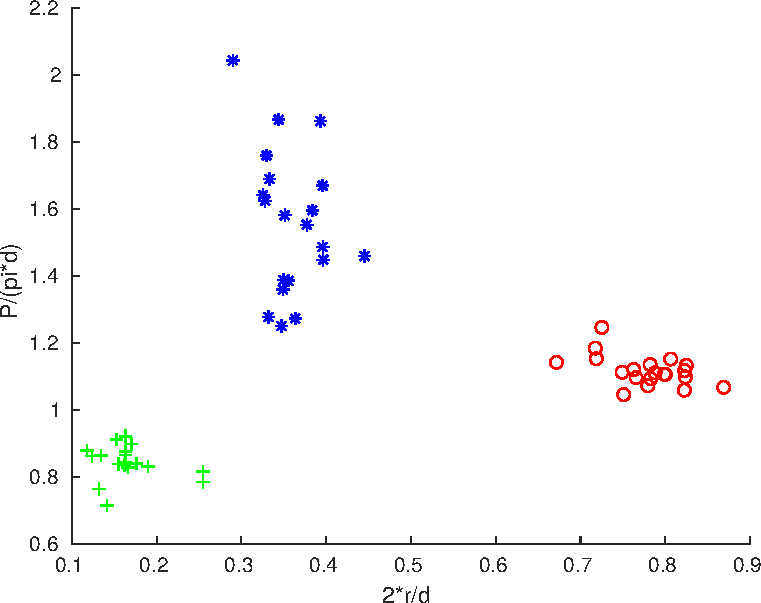
\includegraphics[height=.3\textheight]{diag3.pdf}
 \caption{Three shape diagrams for the three binary images from the Kimia database, and their classification by the kmeans algorithm. The color denotes the real class, and the shape denotes the results of the kmeans algorithm.}
 \label{fig:shape_diagrams:matlab:shapeDiagrams}
\end{figure}

\subsection{Shape classification}
The \matlabregistered{} function \minline{kmeans} is used for classifying the shapes into 3 classes:
\begin{matlab}
X1=x(1,:);
X2=x(2,:);
X3=x(3,:);
Y1=y(1,:);
Y2=y(2,:);
Y3=y(3,:);
idx1 = kmeans([X1',Y1'],3);
idx2 = kmeans([X2',Y2'],3);
idx3 = kmeans([X3',Y3'],3);
\end{matlab}

The classification accuracy for each shape diagram is then computed as a percentage of correctly positioned shapes.
\begin{matlab}
accuracy1 = (sum(idx1(1:20)==mode(idx1(1:20))) + sum(idx1(21:40)==mode(idx1(21:40))) + sum(idx1(41:60)==mode(idx1(41:60))))/60*100
accuracy2 = (sum(idx2(1:20)==mode(idx2(1:20))) + sum(idx2(21:40)==mode(idx2(21:40))) + sum(idx2(41:60)==mode(idx2(41:60))))/60*100
accuracy3 = (sum(idx3(1:20)==mode(idx3(1:20))) + sum(idx3(21:40)==mode(idx3(21:40))) + sum(idx3(41:60)==mode(idx3(41:60))))/60*100
\end{matlab}
with the following results. This quantifies the error done in second diagram (Fig.\ref{fig:shape_diagrams:matlab:shapeDiagrams}).
\begin{mwindow}
accuracy1 = 100
accuracy2 = 98.3333
accuracy3 = 100
\end{mwindow}
